% 2.3.CmakeLibrary.tex
%	Last update: 2019/07/24 F.Kanehori
%newpage
\subsection{cmakeの実行}
\label{subsec:CmakeLibrary}

\noindent
以下では、\cmake の生成物(ビルドの生成物ではありません)を格納する
作業場所(ディレクトリ)を\build として話を進めます(作業場所は任意で構いません)。

\medskip
\noindent
\cmake にはConfigureとGenerateの2段階があります。

\medskip
\noindent
コマンドプロンプトの場合は、1回のコマンドで両方を実行できます。
\Vskip{-.5\baselineskip}
\ifLwarp
	\begin{figure}[h]
	    \begin{center}
	    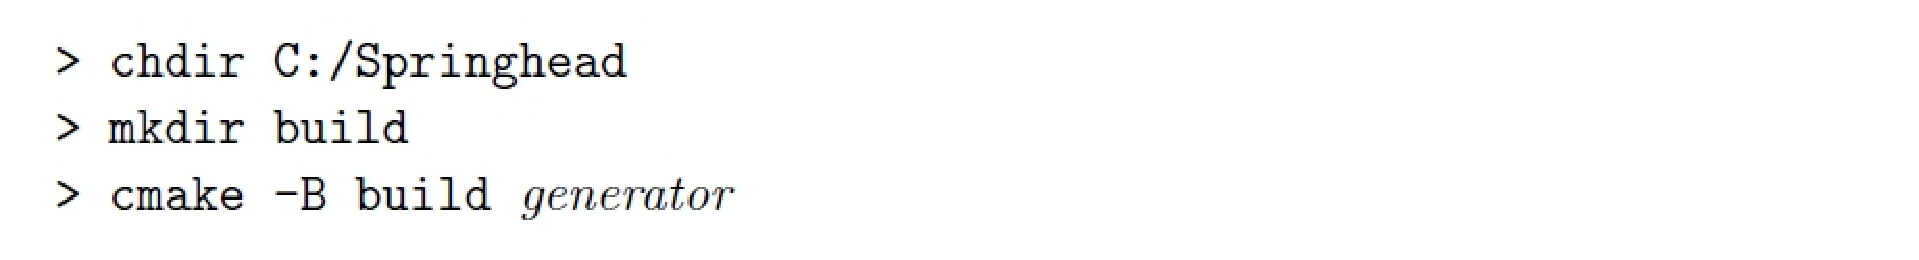
\includegraphics[width=\textwidth]{fig/command-2-3.eps}
	    \end{center}
	    \label{fig:DownloadTree}
	\end{figure}
\else
\begin{narrow}[15pt]
	\CmndBox{%
		> chdir C:/Springhead\\
		> mkdir build\\
		> cmake -B build \it{generator}
	}
	\it{generatorの}詳細(\KQuote{\tt{-G "Visual Studio 15 2017" -A x64}}など)は、
	コマンドプロンプトで\tt{cmake --help}とすると確認できます。
\end{narrow}
\fi

\medskip
\noindent
GUIの場合は、
\begin{narrow}[15pt]
	まずConfigureボタン(図\ref{fig:CmakeConfigure} 左図の下)を押します。
	\begin{figure}[h]
	\begin{center}
	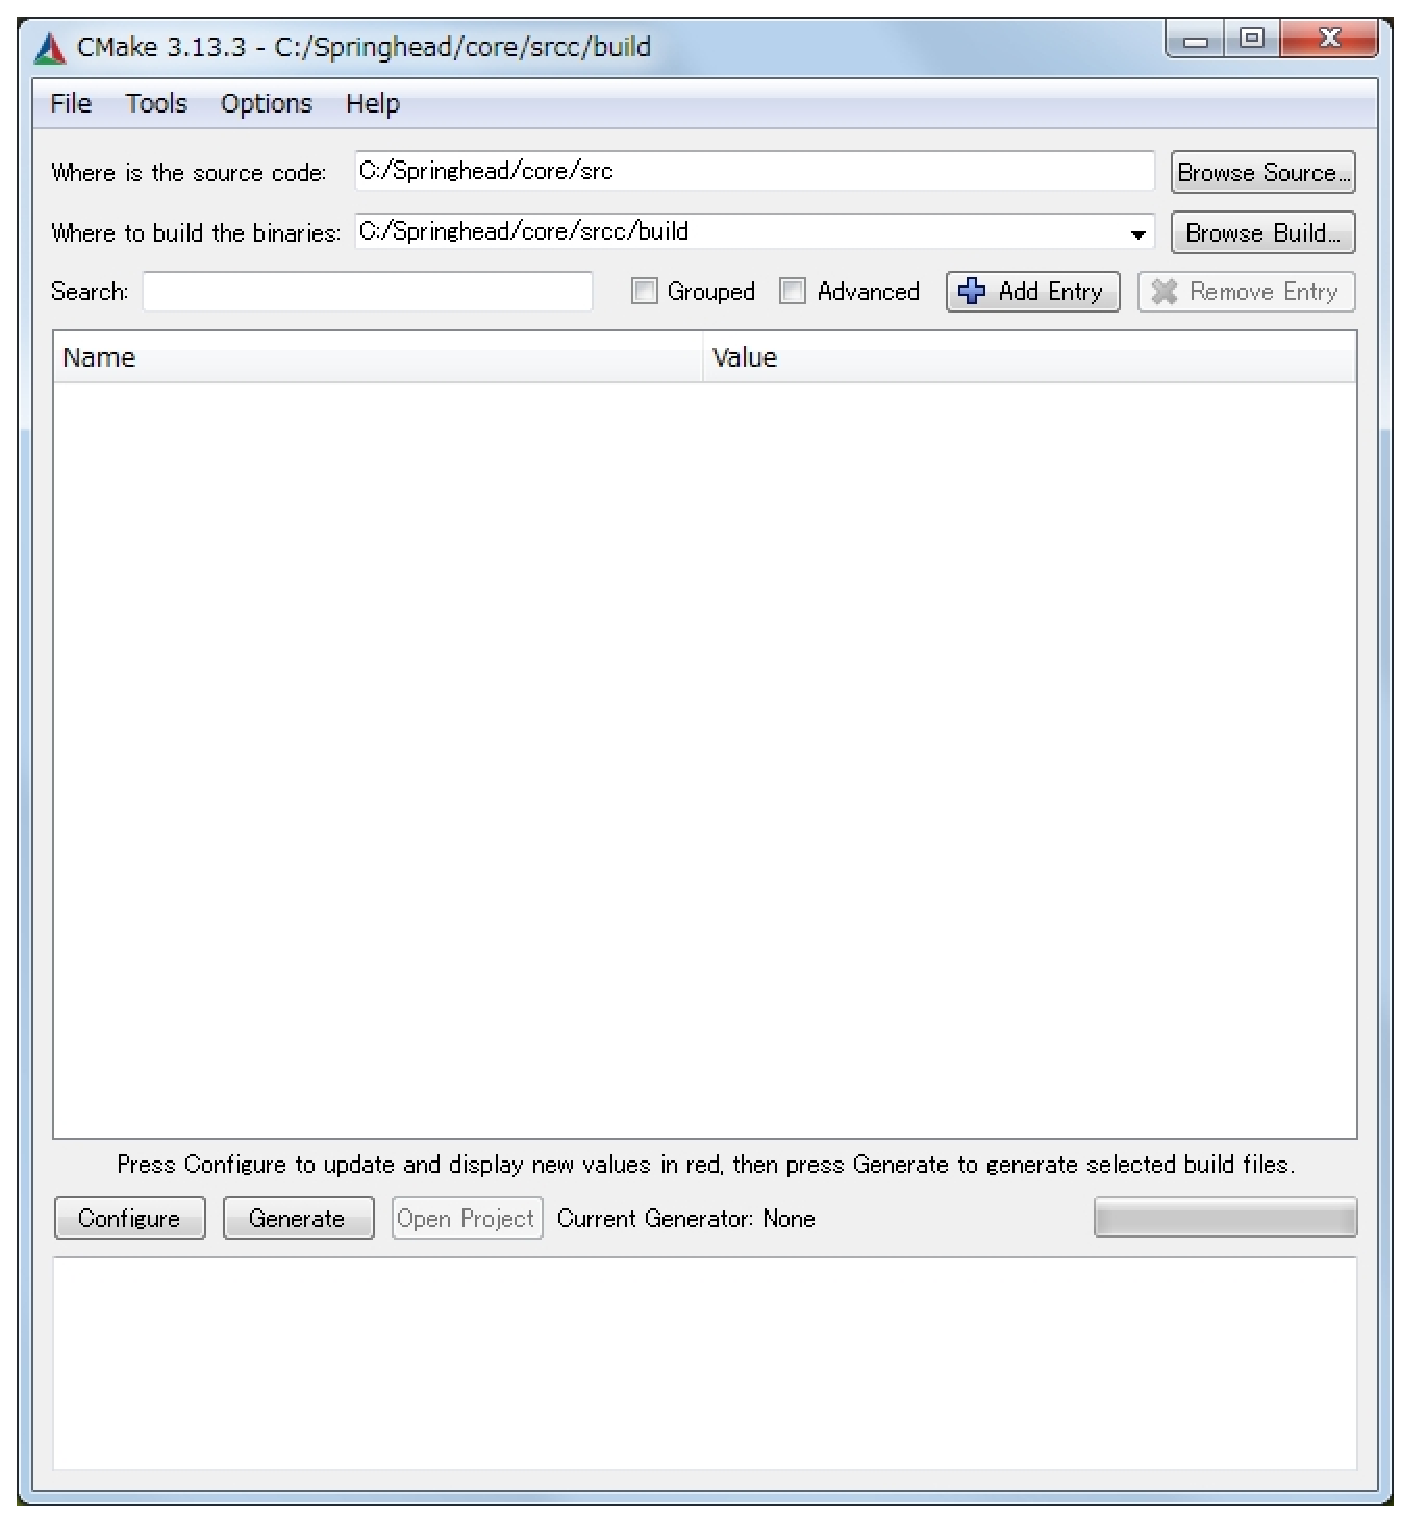
\includegraphics[width=0.35\textwidth]{fig/CmakeConfigure1.eps}
	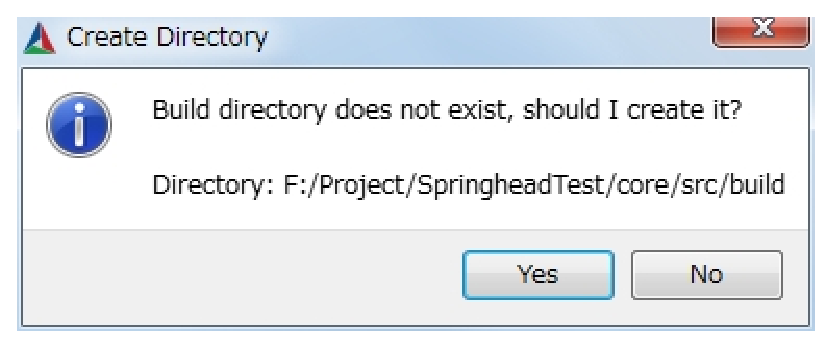
\includegraphics[width=0.2\textwidth]{fig/CmakeConfigure2.eps}
	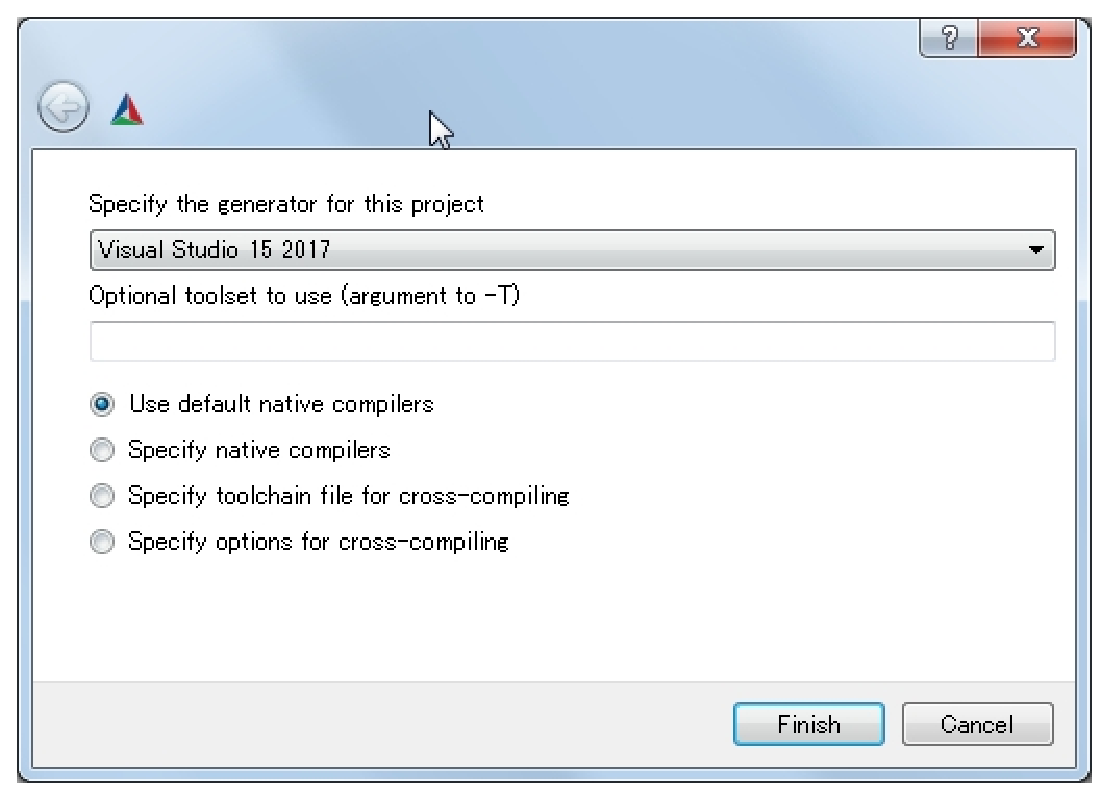
\includegraphics[width=0.3\textwidth]{fig/CmakeConfigure3.eps}
	\end{center}
	\caption{\cmake\ configure}
	\label{fig:CmakeConfigure}
	\end{figure}

	\Vskip{-.5\baselineskip}
	\build ディレクトリがなければ作成するかどうか聞かれ(同中図)、
	次にgenerator指定画面となります(同右図)。
	cmake version 3.15.0では、
	generatorとして図\ref{fig:CmakeGenerator}のものが指定できます。

	\begin{figure}[h]
	\begin{center}
	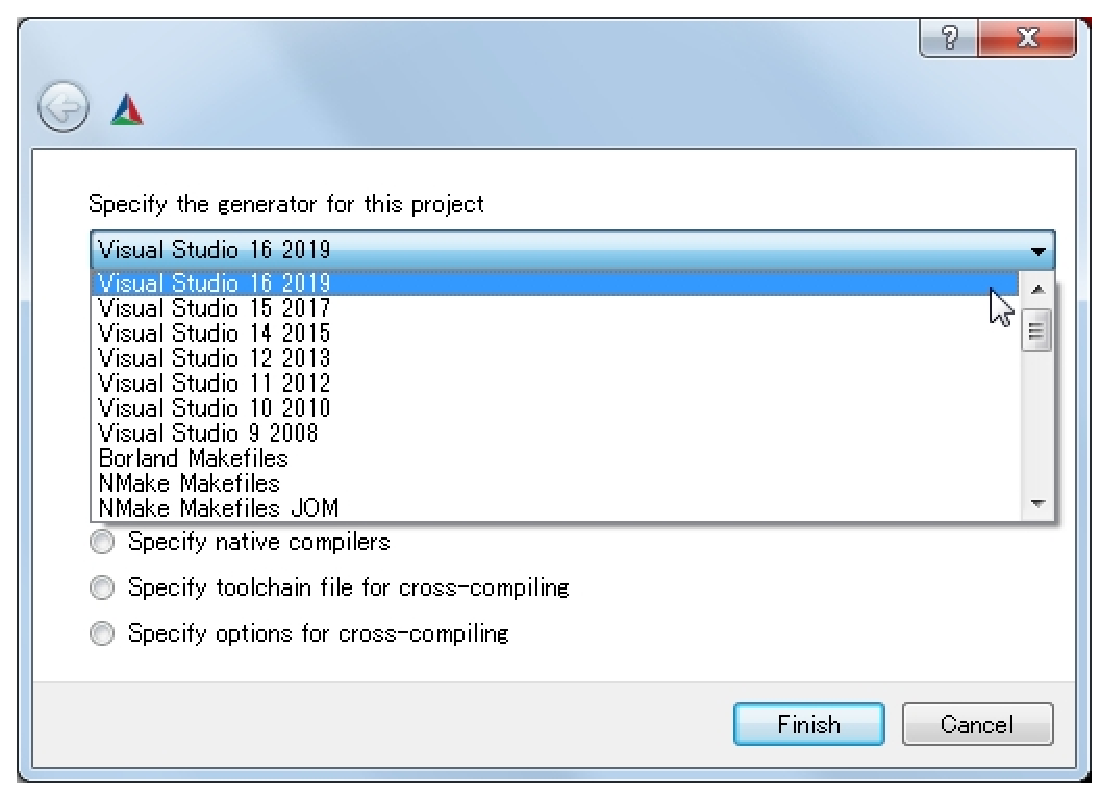
\includegraphics[width=0.3\textwidth]{fig/CmakeConfigure4.eps}
	\end{center}
	\caption{\cmake\ generator}
	\label{fig:CmakeGenerator}
	\end{figure}

	最後に図\ref{fig:CmakeConfigure} 左図下のGenerateボタンを押します。
\end{narrow}

\medskip
\noindent
以上で、\build 以下にsolution/project fileなどが生成されたはずです。

\bigskip

% end: 2.3.CmakeLibrary.tex
